\documentclass[xetex,mathserif,serif]{beamer}
\usepackage{polyglossia}
\setdefaultlanguage[babelshorthands=true]{russian}
\usepackage{minted}
\usepackage{tabu}
\usepackage{moresize}

\useoutertheme{infolines}

\usepackage{fontspec}
\setmainfont{FreeSans}
\newfontfamily{\russianfonttt}{FreeSans}

\definecolor{links}{HTML}{2A1B81}
\hypersetup{colorlinks,linkcolor=,urlcolor=links}

\usepackage{beamerthemesplit} 
\usepackage{wrapfig} 
\usepackage{verbatim} 
\usepackage{pdfpages} 
\usepackage{amsmath} 
\usepackage{cmap}
\usepackage{array} 
\usepackage{amsmath} 
\usepackage{tikz} 
\usepackage{multirow} 
\usepackage[noend]{algpseudocode} 
\usepackage{algorithm} 
\usepackage{algorithmicx} 
\usetikzlibrary{shapes,arrows} 
\usetikzlibrary{calc}
\usepackage{fancyvrb} 
\usepackage{tikz} 
\usepackage{pgfplots} 
\usepackage{sidecap} 
\usepackage{soul}
\usepackage{xcolor}
\usepackage{tabu}
\usepackage{zref-savepos}
\usepackage{colortbl}
\usepackage[normalem]{ulem}

\newcommand{\attribution}[1] {
    \vspace{-5mm}\begin{flushright}\begin{scriptsize}\textcolor{gray}{\textcopyright\, #1}\end{scriptsize}\end{flushright}
}

\beamertemplatenavigationsymbolsempty 

\title[REAL.NET]{Визуальное моделирование --- программирование для непрограммистов}
\institute[CПбГУ]{Санкт-Петербургский государственный университет \\
    Кафедра системного программирования} 

\author[Юрий Литвинов]{Ю.В. Литвинов \newline 
    \textcolor{gray}{\small\texttt{y.litvinov@spbu.ru}}
}

\date{27.04.2022} 

\begin{document} 

    \begin{frame}
        \begin{center} 
            {
\includegraphics[width=1cm]{pictures/SPbGU_Logo.png}} 
        \end{center}
        \titlepage
    \end{frame}

    \begin{frame}
        \frametitle{Начнём с примера}
        \begin{center}
            \url{https://trikset.com/products/trik-studio}
        \end{center}
    \end{frame}

    \begin{frame}
        \frametitle{Как оно работает}
        \begin{itemize}
            \item Существующие языки моделирования (UML, SDL, BPMN, ...) не позволяют исполнять программу
            \item Предметно-ориентированные языки
            \begin{itemize}
                \item Формальные языки программирования
            \end{itemize}
            \item Cоздавать редактор визуального языка вручную слишком сложно
            \item[=>] Следовательно, нужны инструменты быстрой разработки визуальных редакторов
        \end{itemize}
    \end{frame}

    \begin{frame}
        \frametitle{Метамоделирование}
        \begin{center}
            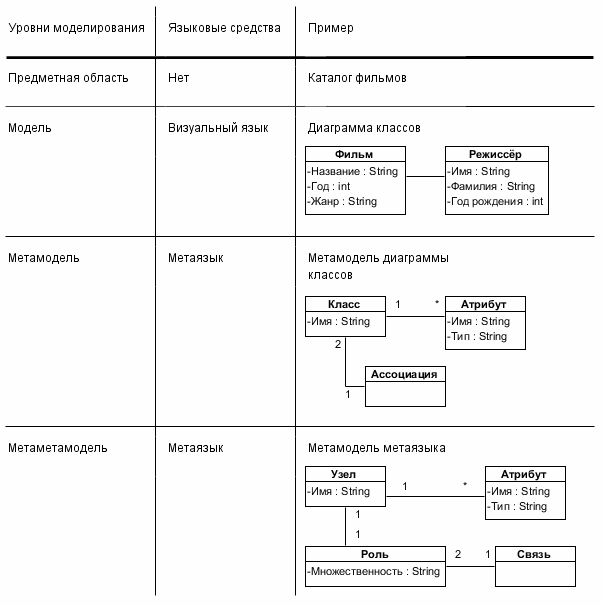
\includegraphics[width=0.6\textwidth]{pictures/metalevels.png}
        \end{center}
    \end{frame}

    \begin{frame}
        \frametitle{QReal}
        \begin{itemize}
            \item 2007 -- где-то 2016
            \begin{itemize}
                \item RTST, RTST++, REAL (с 1980-х до где-то 2002 года)
                \item TRIK Studio активно развивается по сей день
            \end{itemize}
            \item Визуальный метаредактор + редактор форм фигур
            \item Плагинная система
            \item Плагины-редакторы, генерируемые по метамоделям
            \item Плагины-инструменты:
            \begin{itemize}
                \item Генераторы кода, интерпретаторы, версионный контроль и т.п.
                \item Вся TRIK Studio --- это набор языковых плагинов и плагинов-инструментов к QReal
            \end{itemize}
        \end{itemize}
    \end{frame}

    \begin{frame}
        \frametitle{REAL.NET}
        \begin{itemize}
            \item REAL.NET --- платформа для экспериментов над визуальными языками
            \item .NET (C\# + F\#), десктопный и веб-редактор
            \item Неторопливо разрабатывается с 2017 года
            \item Микросервисная архитектура веб-версии
            \item ``Глубокое метамоделирование''
        \end{itemize}
    \end{frame}

    \begin{frame}
        \frametitle{Глубокое метамоделирование}
        \begin{center}
            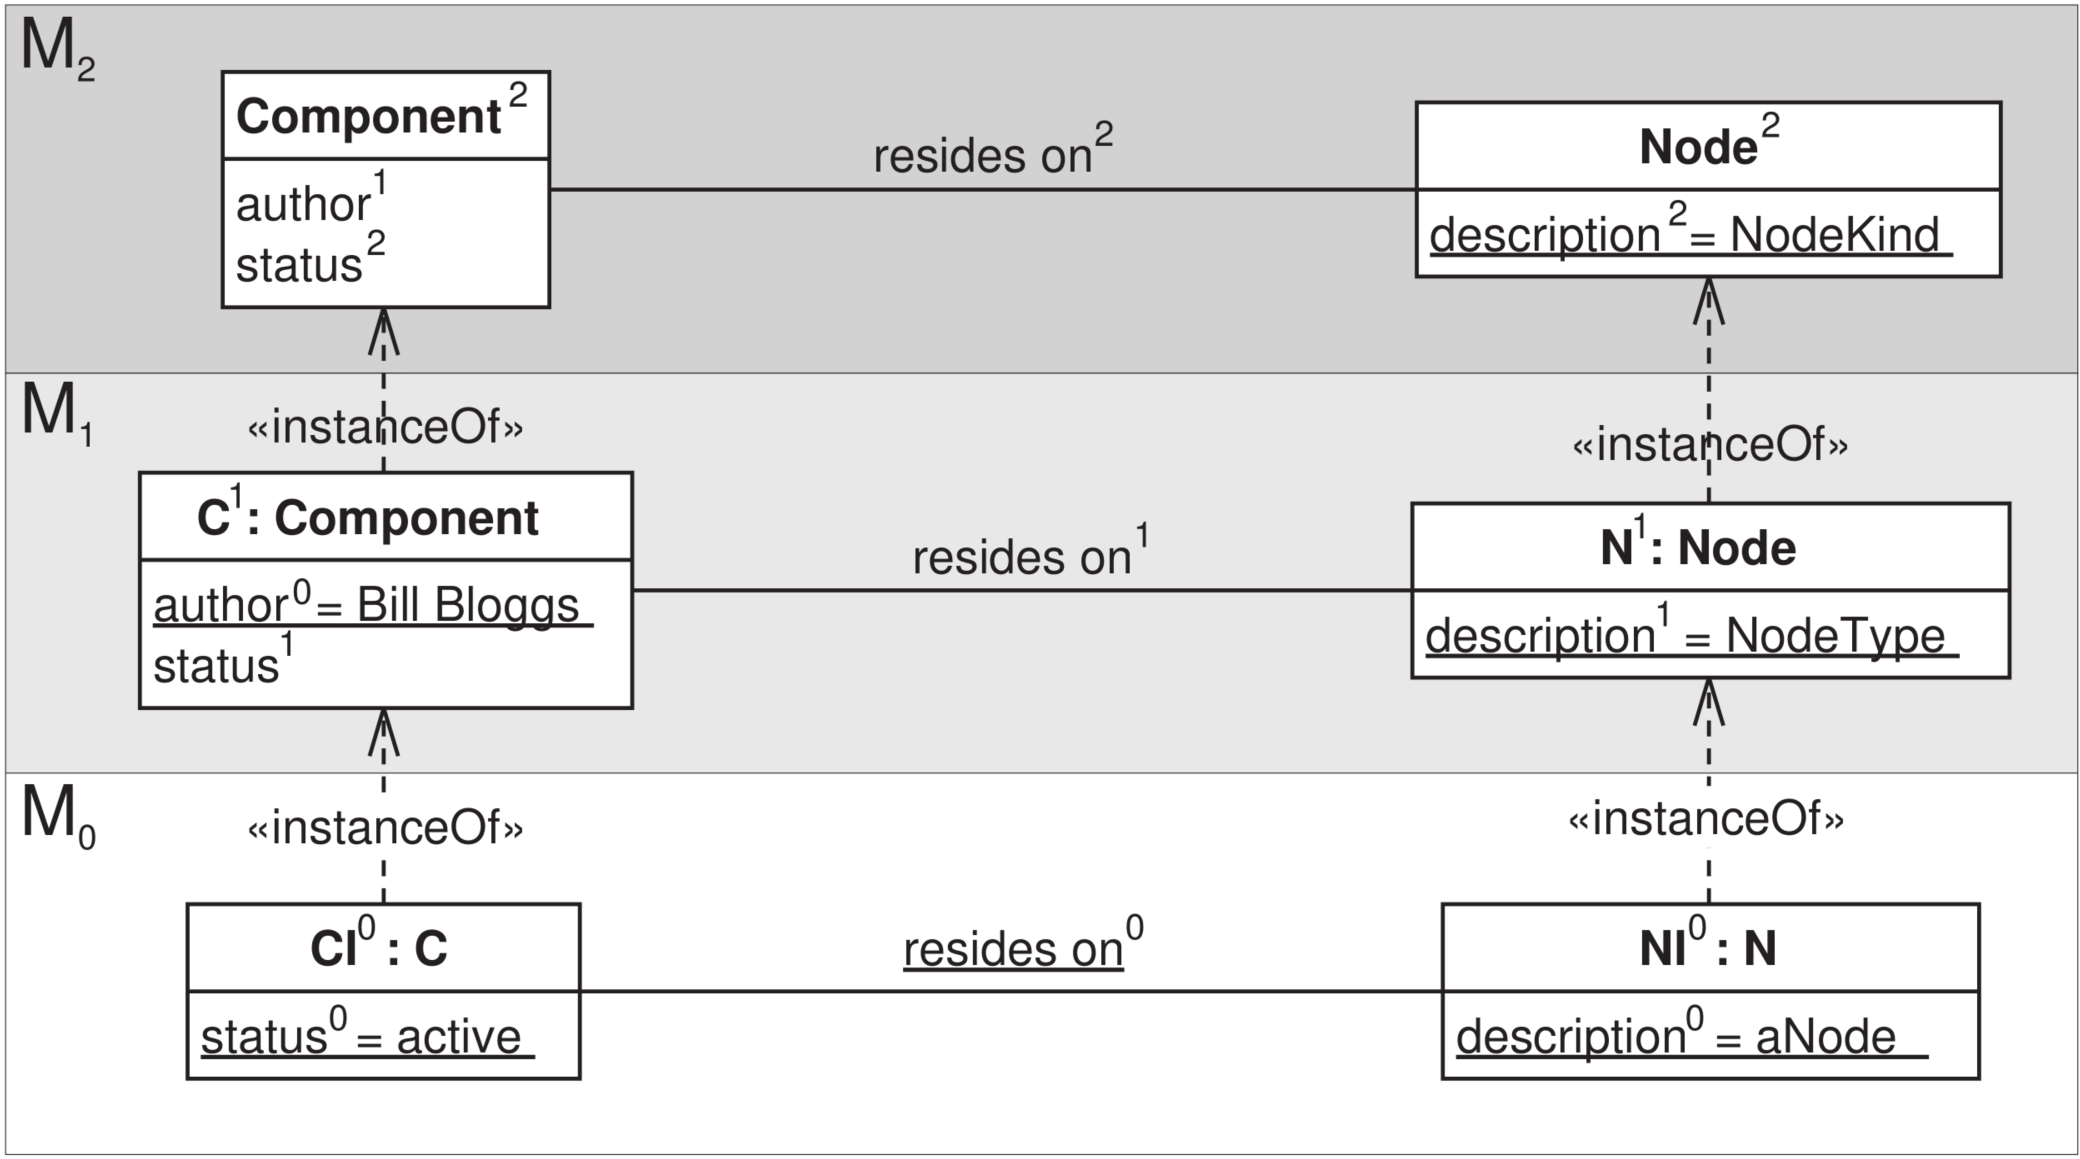
\includegraphics[width=0.8\textwidth]{pictures/deepComponents.png}
            \attribution{C. Atkinson, Th. Kuhne, The Essence of Multilevel Metamodeling, 2001}
        \end{center}
    \end{frame}

    \begin{frame}
        \frametitle{REAL.NET, редактор планов СУБД}
        \begin{center}
            \Large Демо
        \end{center}
    \end{frame}

\end{document}